% arara: xelatex: { shell : yes }
\documentclass[12pt,oneside,a4paper]{book}%one-page printing

%\usepackage[T1]{fontenc}
\usepackage{graphicx}
%\usepackage{setspace}
%\usepackage{epic} % Images drawn in Xfig, exported as .epic
\usepackage{hyperref}
\usepackage[usenames,dvipsnames]{xcolor}
\usepackage{amssymb}
%\usepackage{proof}
%\usepackage{latexsym}
\usepackage{rotating}
%\usepackage{epsfig}
\usepackage{subfigure}
\usepackage{multirow}
\usepackage{titlesec}

\usepackage{enumitem}
\usepackage{cleveref}
\usepackage{pdflscape}
\usepackage{xcolor}
\usepackage[normalem]{ulem}
%\usepackage{index}
%\newindex{default}{idx}{ind}{Index}

\usepackage[section]{placeins}
\usepackage{makecell}
\renewcommand{\cellalign}{l}

\input tex/mepmacro.tex %couple of macros for formatting the mep semestral project,
                    %your personal and specific macros can be placed also there

\titleformat{\chapter}[display]{\normalfont\bfseries}{}{0pt}{\Huge}

%MEP
\newcommand\DissTitle{Case Study: Decision process analysis}
\newcommand\FirstandFamilyName{Radka Bodnarova, Jan Bittner}
\newcommand\Email{bodnarad@fit.cvut.cz, bittnja3@fit.cvut.cz}
\newcommand\Month{Prague, December}
\newcommand\Year{2020}

\newcommand\Department{Department of Software Engineering}
\newcommand\Faculty{Faculty of Information Technology}
\newcommand\University{Czech Technical University in Prague}
\newcommand\Address{Th\'akurova{} 9, 160 00 Prague 6, Czech Republic}

%DEMO commands
\newcommand{\oact}[1]{\textcolor{BrickRed}{#1}}
\newcommand{\iact}[1]{\textcolor{OliveGreen}{#1}}
\newcommand{\dact}[1]{\textcolor{NavyBlue}{#1}}
\newcommand{\btrap}[1]{\textcolor{NavyBlue}{\uline{#1}}}


\begin{document}
% allow @ to appear in macro names
\makeatletter
\coverpagestarts
\newpage
\section*{Abstract}

The goal of this thesis is to analyse a part of the law about judgement issuing. We analyzed the law using OER method while focusing on ontological transactions. While analyzing the text and constructing transaction tables, we discovered that a lot of things are mising or things are tacid. From the tables we created Interaction Structure Model diagram, OCD diagram and OFD diagram. A part of the analyzed model was modeled in BPMN in Camunda platform.

\bigskip

\noindent{\bf Keywords:}

~Judgement issuing, DEMO methodology, BPMN model, process execution

\vfill

%This is not mandatory, but please, please, please keep it here, it means a lot to our research at the CCMi. 
\section*{License}
The authors agree to publish this work under the \href{https://creativecommons.org/licenses/by/4.0/}{Creative Commons 4.0 license} and help the ongoing scientific research at the CCMi FIT CVUT in Prague. 
\newpage
\tableofcontents
\mainbodystarts

%  Chapters start here
\chapter{Organization Essence Revealing}

The goals of this chapter are to perform an OER analysis as described in~\cite{dietz2015teoo,dietz2020enterprise}. For simplicity, we will only do the following steps: 

\begin{enumerate}
    \item Insert the project domain description into this document. 
    \item Perform the OER analysis and find \oact{ontological acts}. Be vigilant about the \btrap{blue traps}!
    \item Identify ontological transaction kinds and put them in the text. E.g. \oact{[TK1/rq]} If there are not enough red transactions, you can include the green ones. 
    \item Create an extended transaction result table (e-TRT). Map the transaction acts to the project domain description. See the~\cref{tab:etrt}. 
    \item Create a Subject-Actor table to realize the distinction between roles and DEMO actor roles. See the~\cref{tab:subjectactortable}. 
    \item Think in trees, not in flows and create the interaction structure of your transaction kinds. See the~\cref{fig:interactionStructure}.  
    \item Produce the Coordination Structure Diagram (CSD) and the Object Fact Diagram (OFD). See the~\cref{fig:csdModel} and ~\cref{fig:ofdModel}.  
    \item Finally, summarize your modeling thoughts and revelations. Don't forget about missing transaction steps table~\cref{tab:missing_transaction_steps}. 
\end{enumerate}

The process description of the Volley Case and it's OER analysis was taken from the Enterprise Ontology book~\cite{dietz2020enterprise}. 

%In the step 1 a coloring of the process description is made. The coloring can be done on text as well as on the flow chart diagram. 
\section{OER Step 1: Distinguishing Performa-Informa-Forma}

Legend: 
\begin{itemize}
    \item \oact{Ontological Act [Transaction Kind/Act type]}
    \item \btrap{Blue trap ontological act}!
\end{itemize}

\paragraph{\S 1 Preliminary Rules}

\begin{enumerate}[label={(\arabic*)}]
\item One can \oact{become member of the tennis club Volley[TK1]} by \btrap{sending a letter}\oact{[TK1/rq]} to the club by postal mail. In the letter one has to mention \iact{one’s surname and first name, birth date, gender, telephone number, and postal mail address (street, house number, zip code, and town)}. Adam, the administrator of Volley, \dact{empties the mailbox} daily and checks whether the information provided is complete. If not, he \dact{makes a telephone call} to the sender in order \iact{to complete the data}. Once a letter is complete, Adam \dact{writes an incoming mail number and the date on the letter, records the letter in the letter book, and puts it in a folder}. 
\item Every Wednesday evening, Adam \dact{takes the folder} to Eve, the secretary of Volley. He also \dact{takes the member register with him}. If Eve \oact{decides that an applicant can become member of Volley[TK1/pm]}, \dact{she stamps ‘new member’ on the letter and writes the date below it. She then hands the letter to Adam in order to add the new member to the member register. This is a book with numbered lines. Each new member is entered on a new line. The line number is the number by which the new member is referenced in the administration}. Next, Eve \iact{calculates the fee} that the new member \oact{has to pay [TK2]} for the remaining part of the calendar year. She asks Adam for the \iact{annual fee}, as \oact{decided at the general assembly [TK out of scope]}, which Adam \dact{has recorded on a sheet of paper}. Then, she asks Adam to \dact{write down the amount in the member register}. 
\item If Eve \oact{does not allow an applicant to become member[TK1/dc]} (e.g. because he or she is too young or because the maximum number of members has been reached), Adam will \btrap{send a letter}\oact{[TK2/rq]} in which he \iact{explains why the applicant cannot (yet) become member of Volley}.
\end{enumerate}

\paragraph{\S 2 Some Other Rules}

\begin{enumerate}[label={(\arabic*)}]
\item When all applications are processed, Adam \dact{takes the letters and the member register home} and \iact{prepares an invoice} to all new members for the \oact{payment of the first fee[TK2]}. He \btrap{sends these invoices}\oact{[TK2/rq]} \dact{by postal mail}. Payments have to be performed by bank transfers.
\item As soon as \btrap{a bank statement is received}\oact{[TK2/da]}, Adam \dact{prints a card} on which \iact{the member number, the starting date, the name, the date of birth, the gender, and the residence} are mentioned. \btrap{The card is sent}\oact{[TK1/da]} \dact{to the new member by postal mail}.
\end{enumerate}





\begin{landscape}
\section{OER Step 2: Identifying Transaction Kinds and Actor Roles}

\begin{table}[h]
\caption{Extended Transaction Result Table}
\label{tab:etrt}
\begin{tabular}{|l||l|l|}
\hline
Transaction  & Membership Starting (TK1) & Membership Paying (TK2) \\ \hline
Product      & membership is started  & the first fee of membership is paid \\ \hline
Initiator      & Aspirant Member (AR1)   &  Membership Starter (AR2)\\ \hline
Executor       & Membership Starter (AR2) & Membership Payer (AR3)       \\ \hline
Request        & Sending a letter (\S1/1)  & Sends the invoices (\S2/1)   \\ \hline
Promise        &  Application decision  (\S1/2)  &  Not Specified (Probably Tacit)   \\ \hline
Decline        &  Does not allow an applicant to become member (\S1/3)  & Not Specified  \\ \hline
Declare        & The card is sent to the member (\S2/2) & A bank statement is received  (\S2/2) \\ \hline
Reject         &  Not Specified             &  Not Specified   \\ \hline
Accept         & Not Specified (Probably Tacit) &  Not Specified (Probably Tacit) \\ \hline
Revoke Request & Not Specified                   & Not Specified        \\ \hline
Revoke Promise & Not Specified                   &  Not Specified       \\ \hline
Revoke Declare & Not Specified                    &  Not Specified      \\ \hline
Revoke Accept  &  Not Specified             &   Not Specified             \\ \hline
\end{tabular}
\end{table}

\begin{table}[h]
\caption{Subject Actor Table}
\label{tab:subjectactortable}
\begin{tabular}{|l|l|l|l|}
\hline
  & Aspirant Member (AR1)       & Membership Starter (AR2)  & Membership Payer (AR3)  \\ \hline
Administrator   &  & X  &   \\ \hline
Customer & X &  & X \\ \hline
\end{tabular}
\end{table}

\end{landscape}

\section{OER Step 3: Composing the Essential Model}

Before starting with a CSD model, it is important to think about the transaction interaction structure. The transaction have to form one or more trees to compose into a process. You can see an example in~\cref{fig:interactionStructure}. 

\begin{figure}[h]\centering
	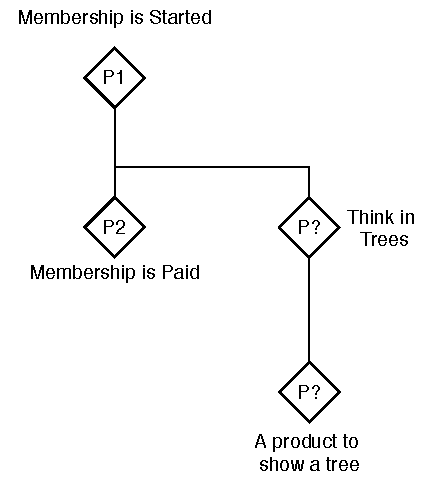
\includegraphics[width=8cm]{pic/VolleyInteractionStructure}
	\caption{An Interaction Structure Model of Volley}
	\label{fig:interactionStructure}
\end{figure}

\begin{figure}[h]\centering
	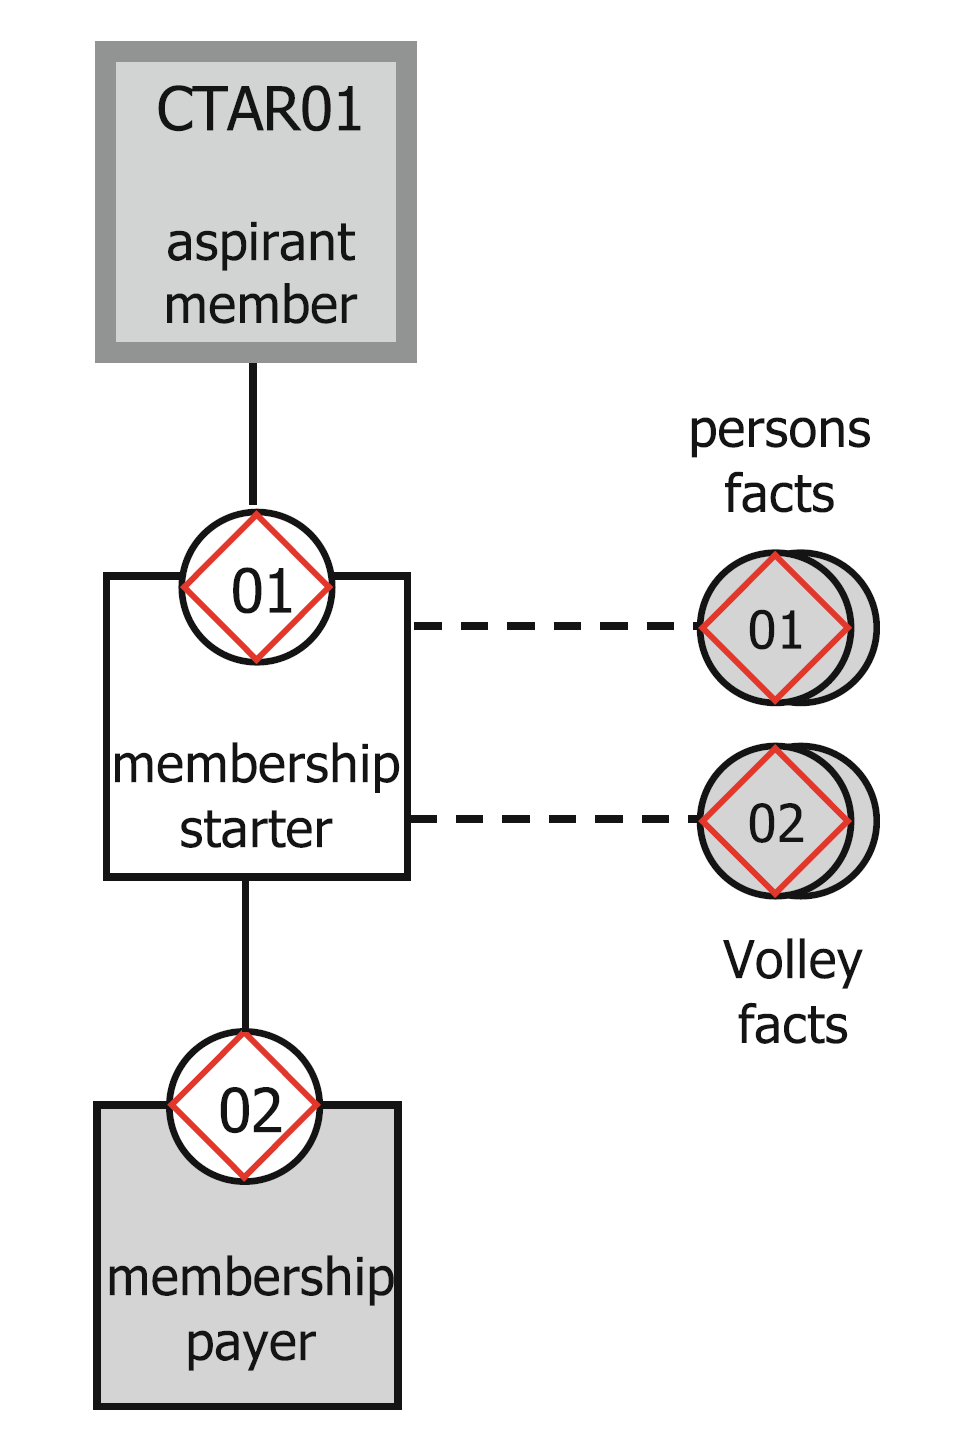
\includegraphics[width=6cm]{pic/VolleyCSD}
	\caption{A CSD Model of Volley~\cite{dietz2020enterprise}}
	\label{fig:csdModel}
\end{figure}

\begin{figure}[h]\centering
	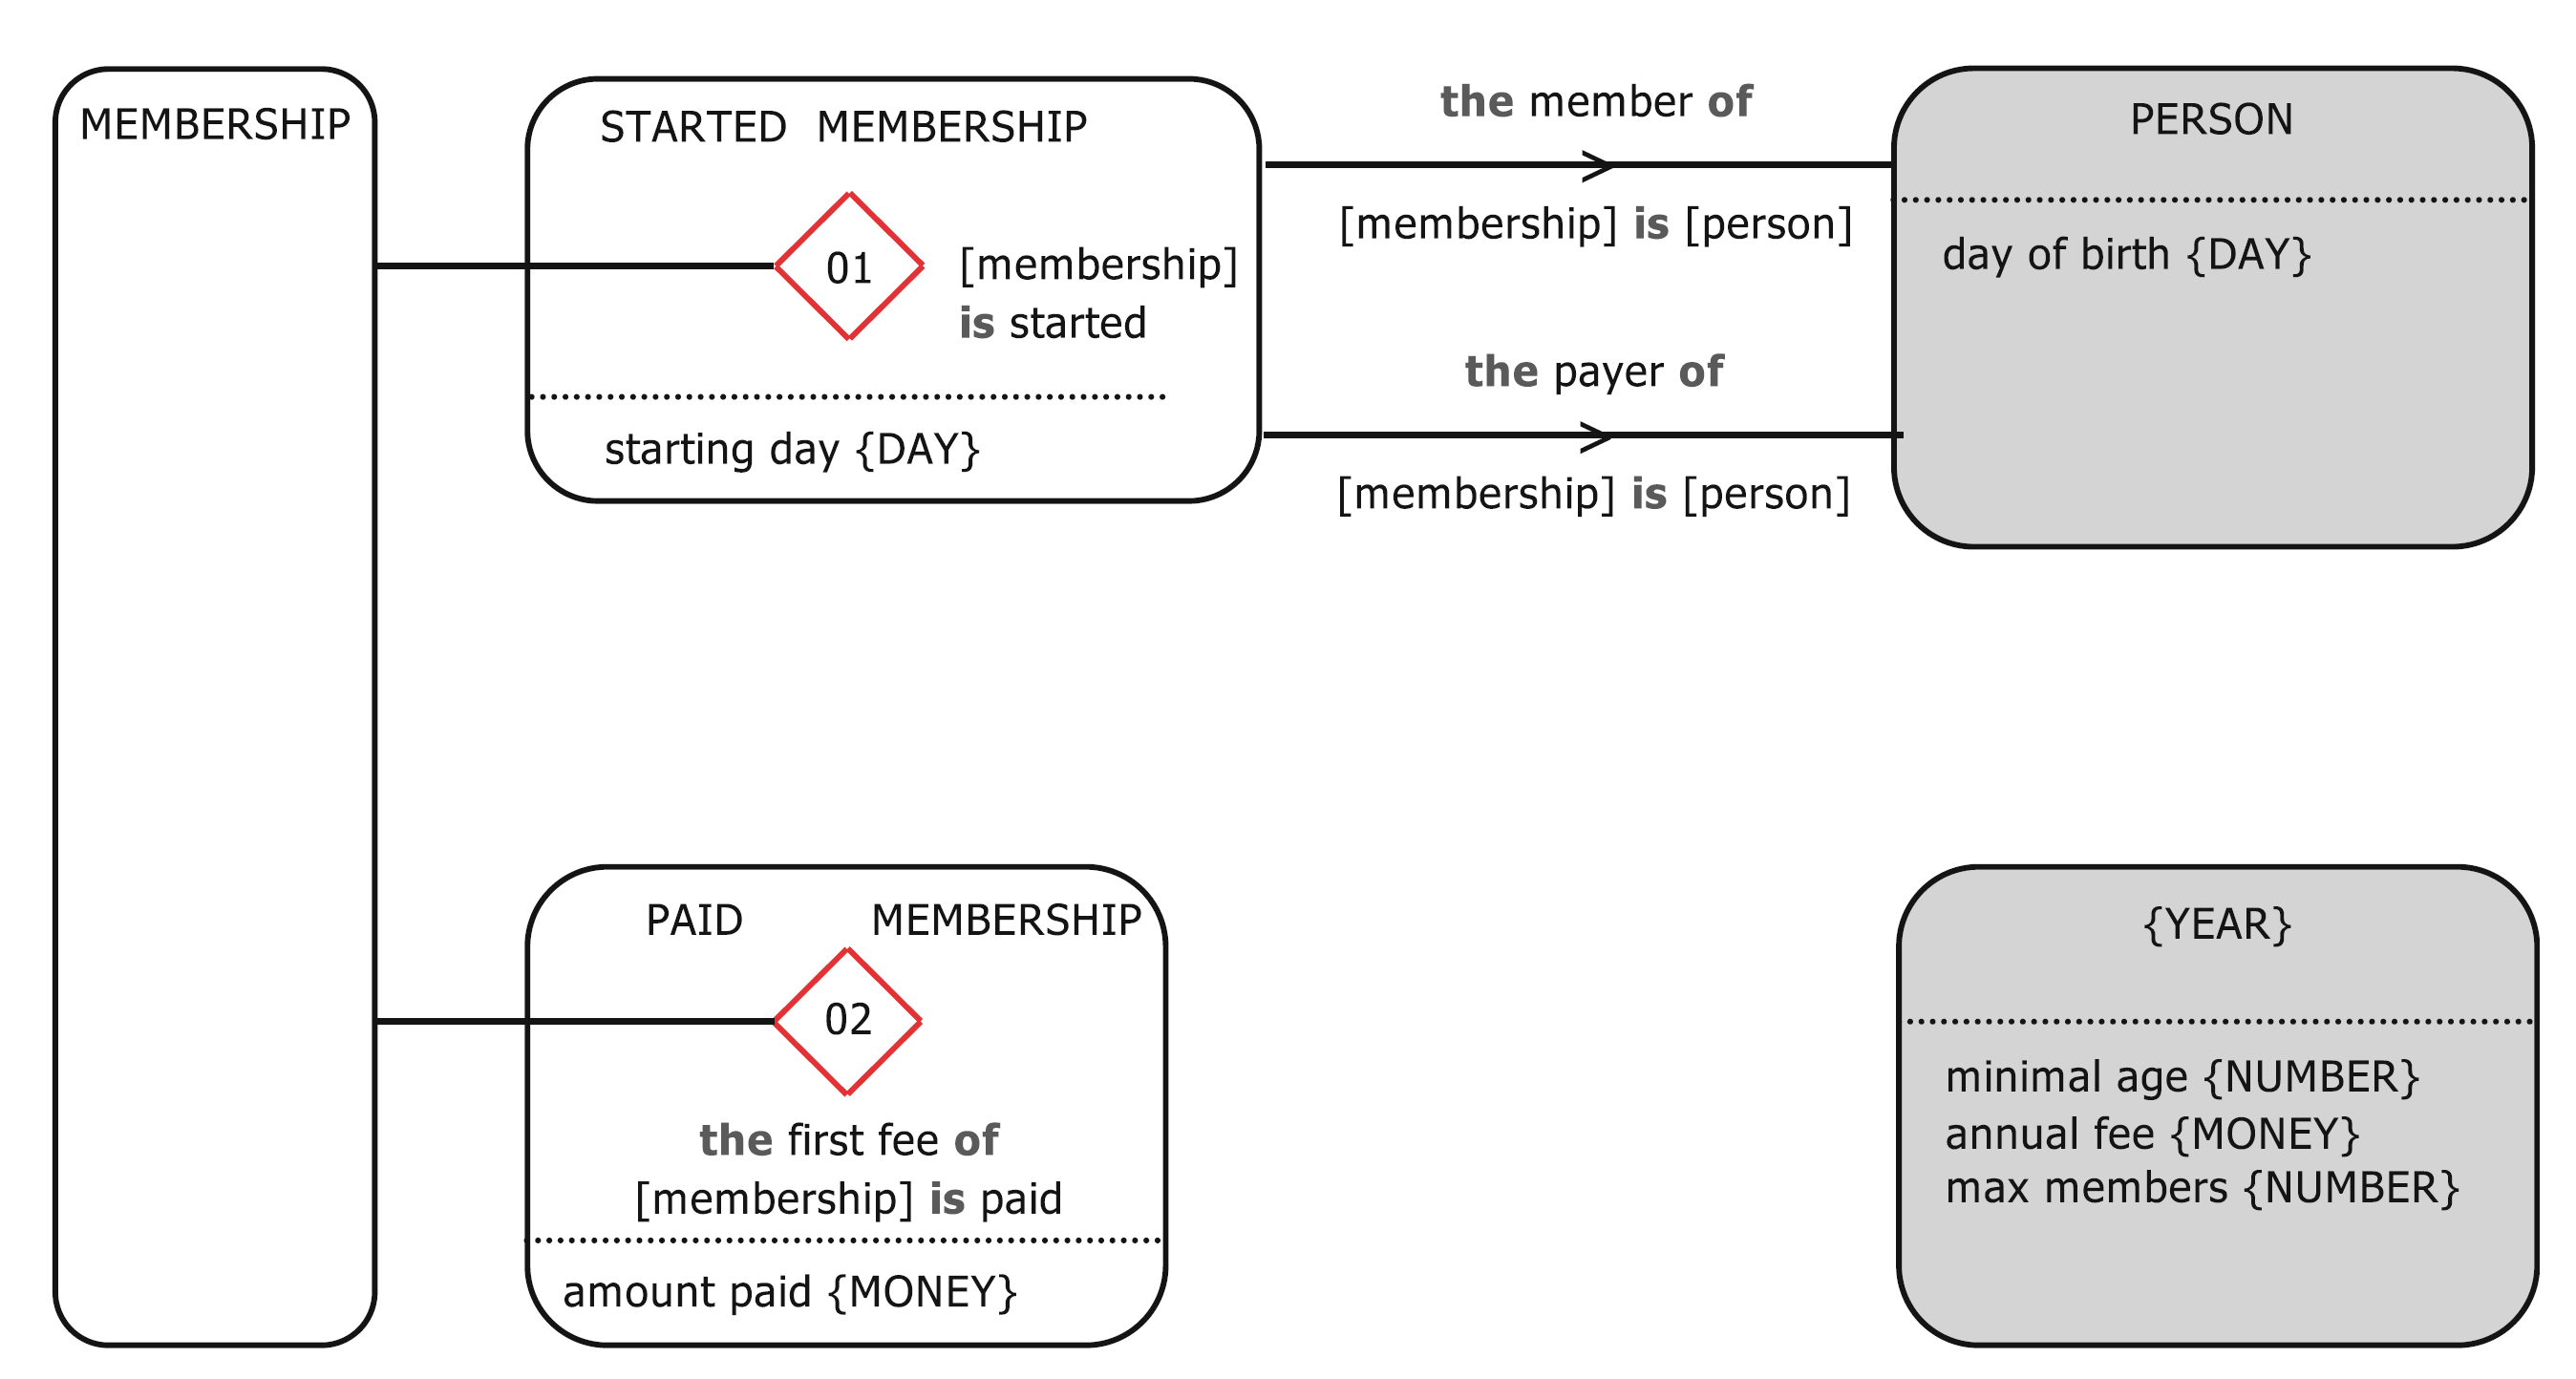
\includegraphics[width=12cm]{pic/VolleyOFD.png}
	\caption{An Object Fact Diagram of Volley~\cite{dietz2020enterprise}}
	\label{fig:ofdModel}
\end{figure}


\section{Summary}

Some comments about the OER analysis belong here. Why were you not able find some responsibilities? What was vaguely defined? Just roast the authors of the assignment (not the teachers :). 

And finally, show how much information is missing in a table~\cref{tab:missing_transaction_steps}. 

\begin{table}[h]\centering
\caption{Missing Transaction Steps}
\label{tab:missing_transaction_steps}
\begin{tabular}{|l||l|l|l|}
\hline
                      & Specified    & Not Specified & Missing Information \\ \hline
\multicolumn{4}{|c|}{Standard Transaction Pattern}                        \\ \hline
Request               & 2           & 0            & 0\%             \\ \hline
Promise               & 1           & 1            & 50\%            \\ \hline
Decline               & 1          & 1           & 50\%             \\ \hline
Declare               & 2           & 0            & 0\%              \\ \hline
Reject                & 0            & 2           & 100\%             \\ \hline
Accept                & 0           & 2            & 100\%            \\ \hline
\textbf{Total}        & \textbf{6} & \textbf{6}  & \textbf{50\%}   \\ \hline
\multicolumn{4}{|c|}{Revokes}                                             \\ \hline
Revoke Request        & 0            & 2           & 100\%             \\ \hline
Revoke Promise        & 0            & 2           & 100\%             \\ \hline
Revoke Declare        & 0            & 2           & 100\%            \\ \hline
Revoke Accept         & 0            & 2           & 100\%             \\ \hline
\textbf{Total}        & \textbf{0}   & \textbf{8} & \textbf{100\%}    \\ \hline
\multicolumn{4}{|c|}{Complete Transaction Pattern}                        \\ \hline
\textbf{Total}        & \textbf{6} & \textbf{14} & \textbf{70\%}    \\ \hline
\end{tabular}

\end{table}
\chapter{Process Automation}

\section{Process Design}

We selected main features of this part of the law and designed BPMN model.

\begin{landscape}

    \begin{figure}[h]\centering
        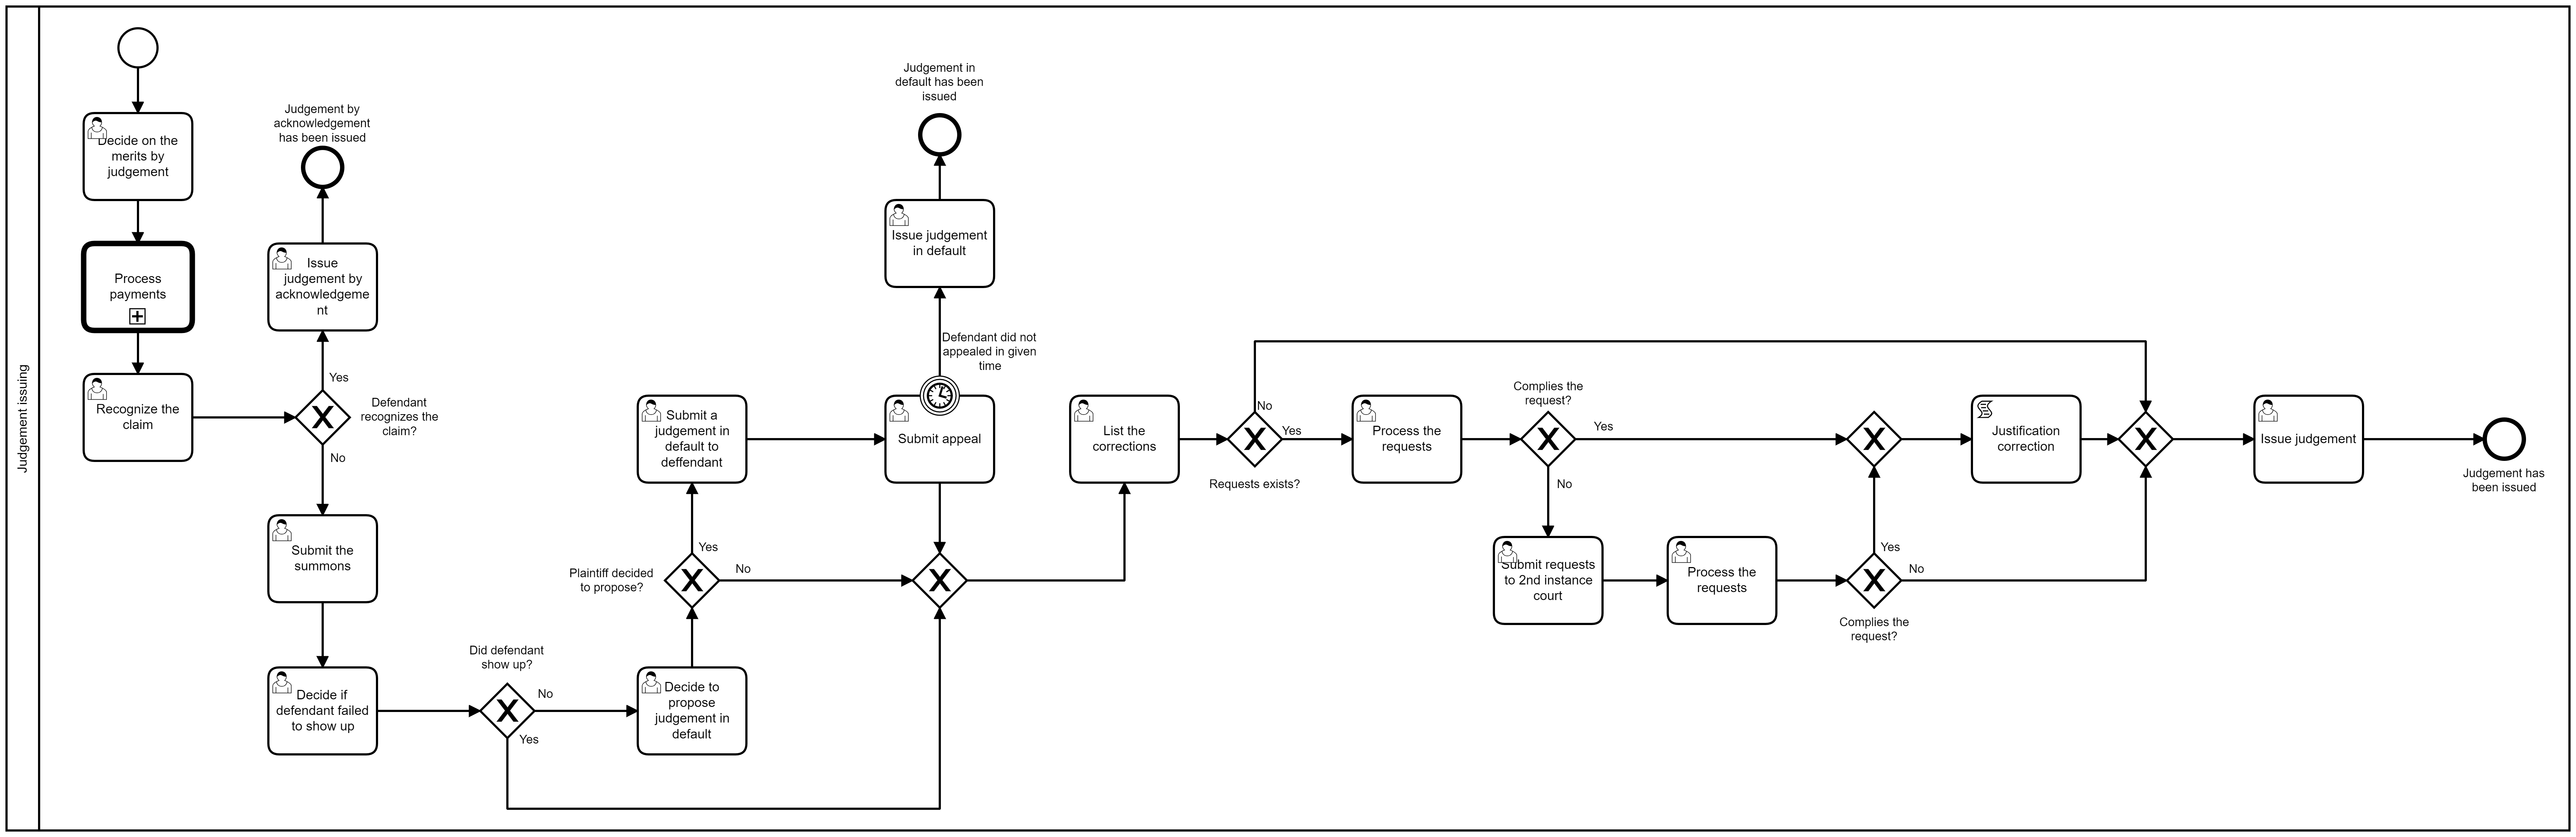
\includegraphics[width=22cm]{pic/bpmn}
        \caption{BPMN main diagram}
        \label{fig:bpmnModel}
    \end{figure}
    
    \begin{figure}[h]\centering
        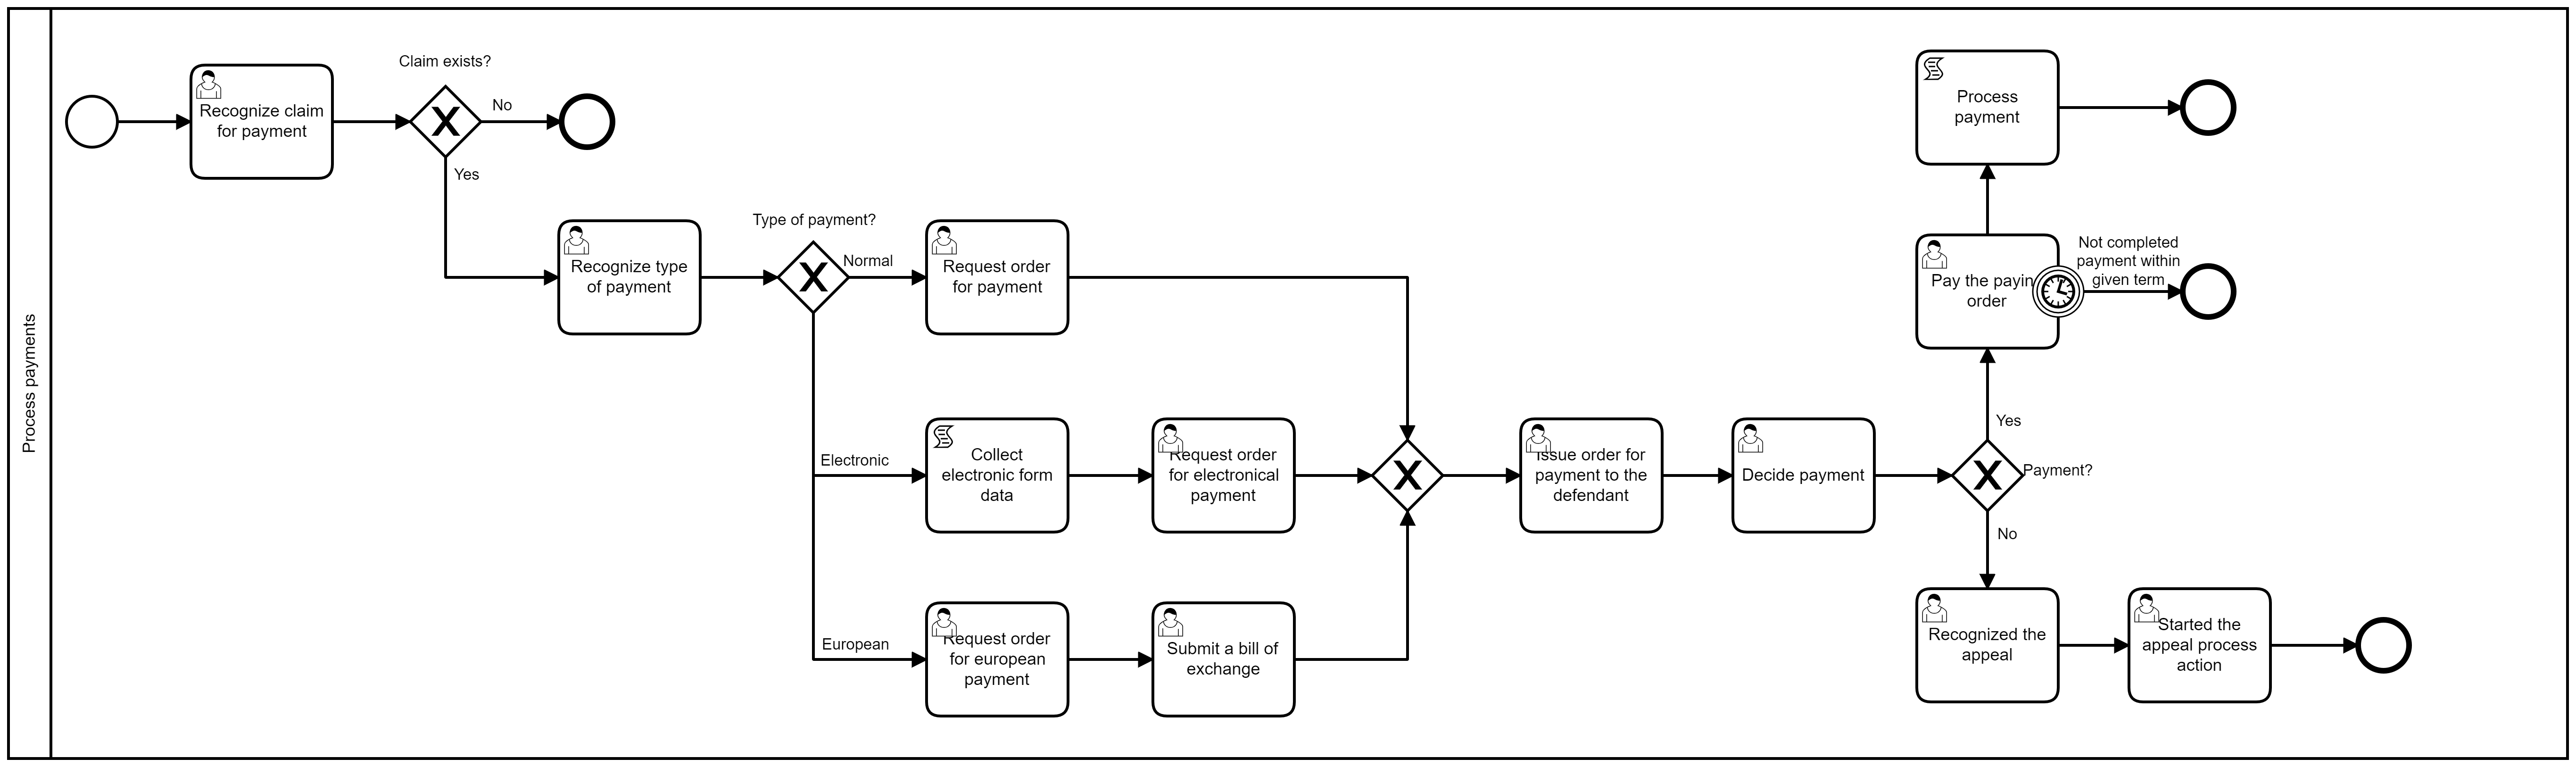
\includegraphics[width=22cm]{pic/bpmn_payments}
        \caption{BPMN payments diagram}
        \label{fig:bpmnPaymentsModel}
    \end{figure}
    
    \end{landscape}
    
    \section{Process Execution}
    
    We also tested the BPMN model in Camunda platform. Figures below shows some of the steps of the process.

    To execute BPMN in Camunda, you need to copy \verb+bodnarova-bittner-forms/+ directory into \verb+./camunda-bpm-tomcat-7.14.0\server\apache-tomcat-9.0.36\webapps+ directory.
    
    \begin{landscape}
        
        \begin{figure}[h]\centering
            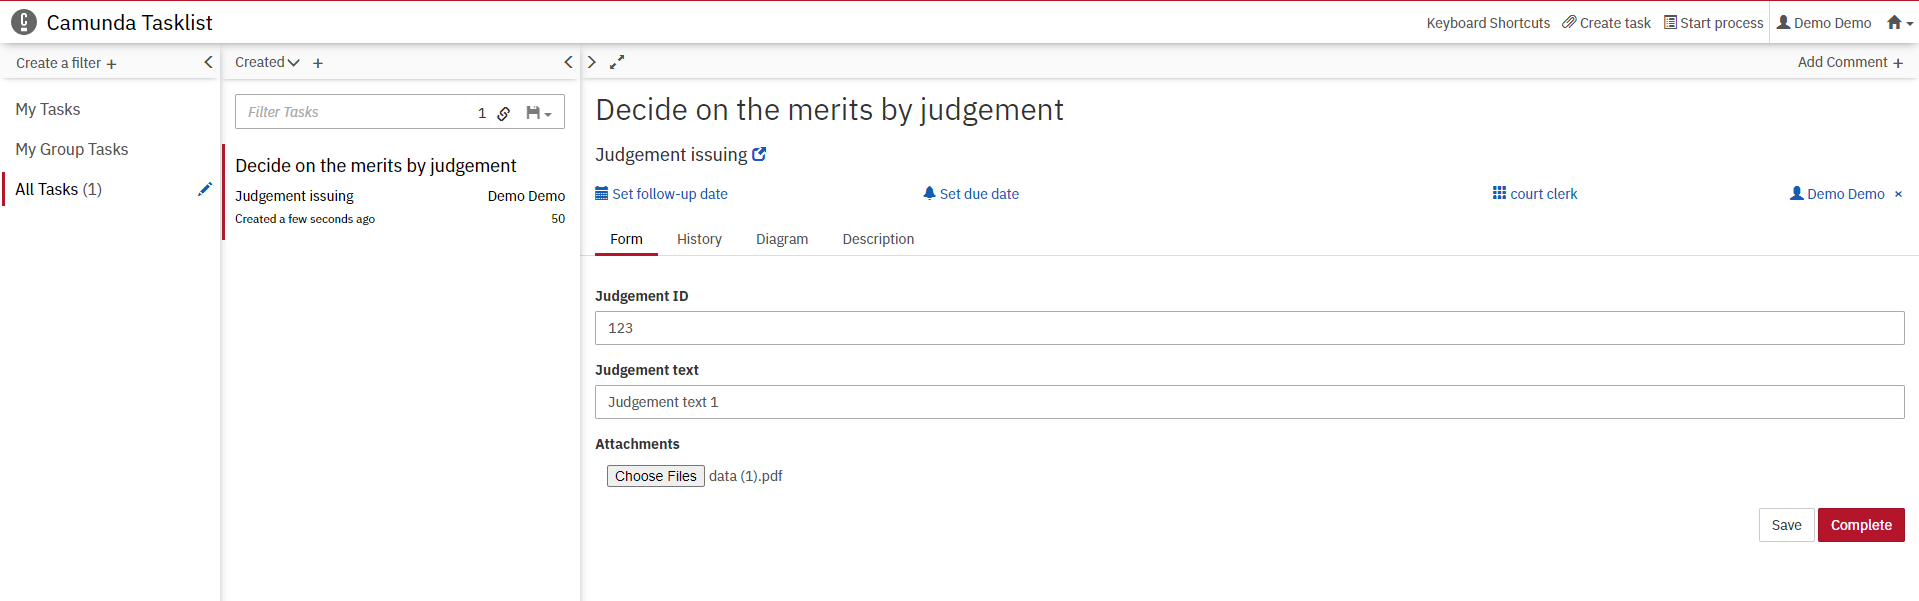
\includegraphics[width=22cm]{pic/camunda1}
            \caption{BPMN form: decide on the merits by judgement}
            \label{fig:camunda1}
        \end{figure}
    
        \begin{figure}[h]\centering
            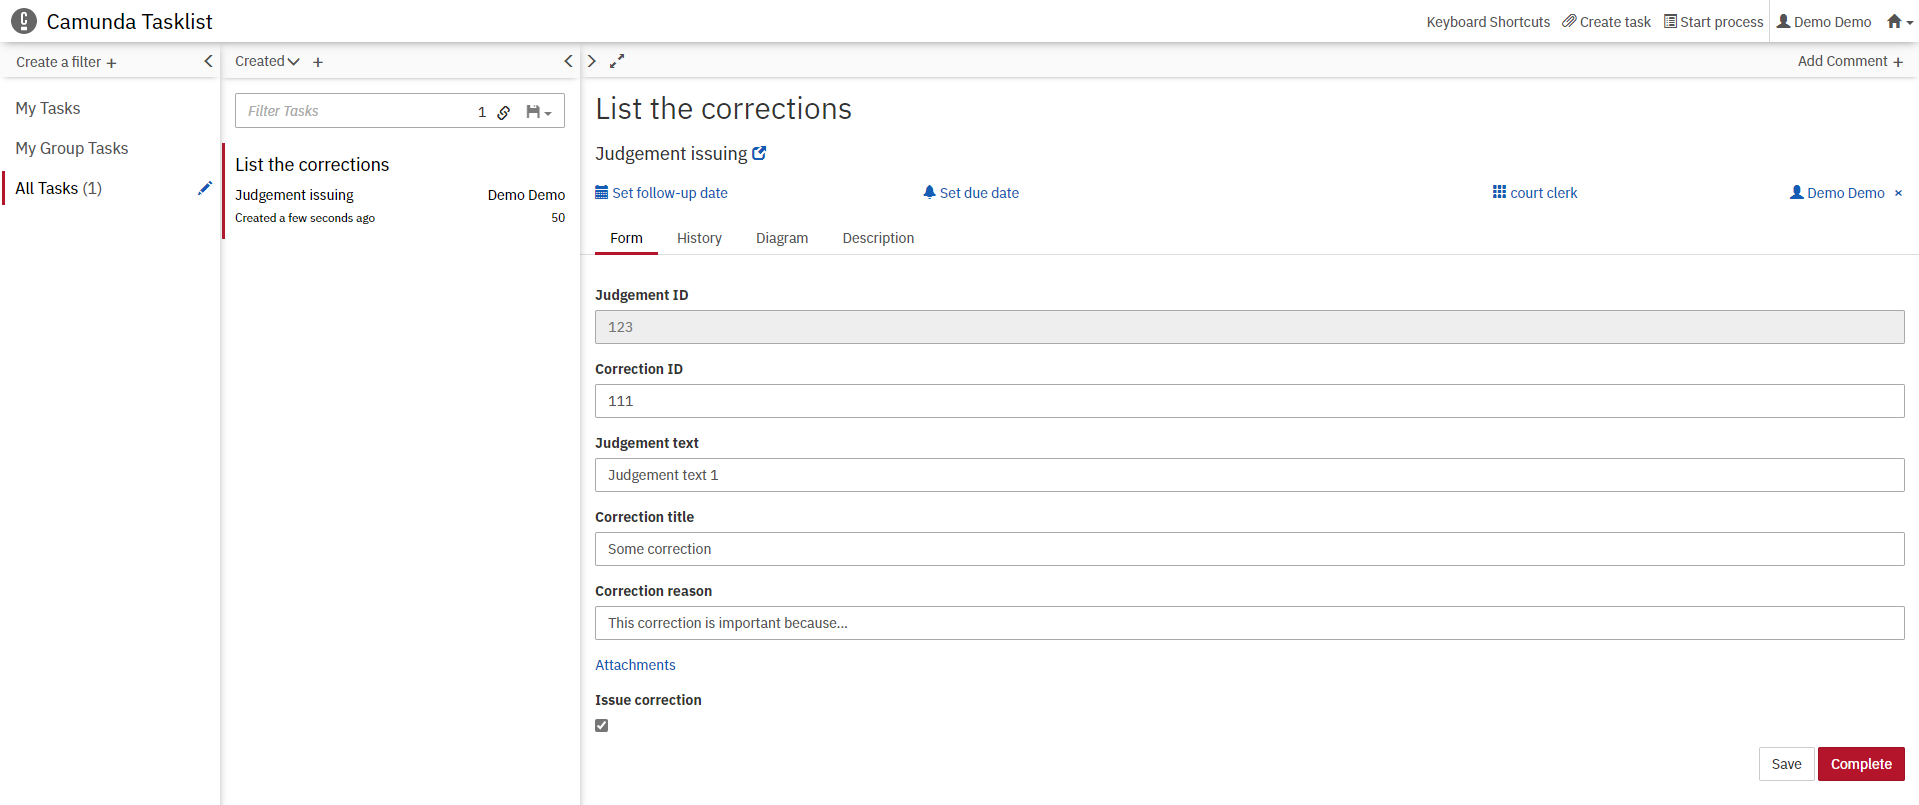
\includegraphics[width=22cm]{pic/camunda2}
            \caption{BPMN form: list the corrections}
            \label{fig:camunda2}
        \end{figure}
    
        \begin{figure}[h]\centering
            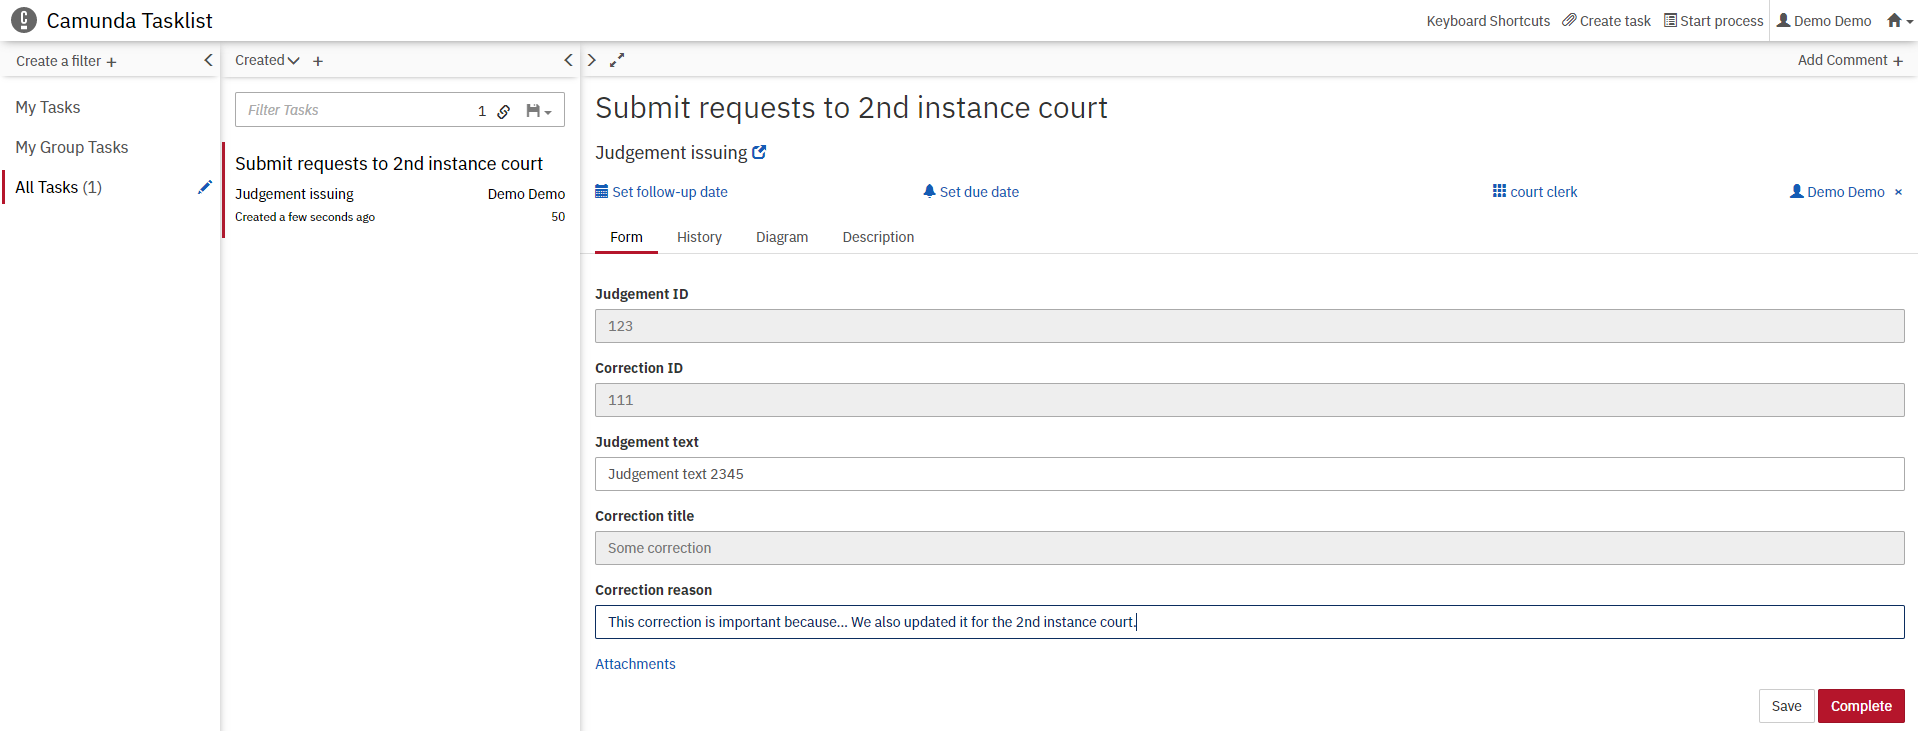
\includegraphics[width=22cm]{pic/camunda3}
            \caption{BPMN form: submit requests to 2nd instance court}
            \label{fig:camunda3}
        \end{figure}
    
        \begin{figure}[h]\centering
            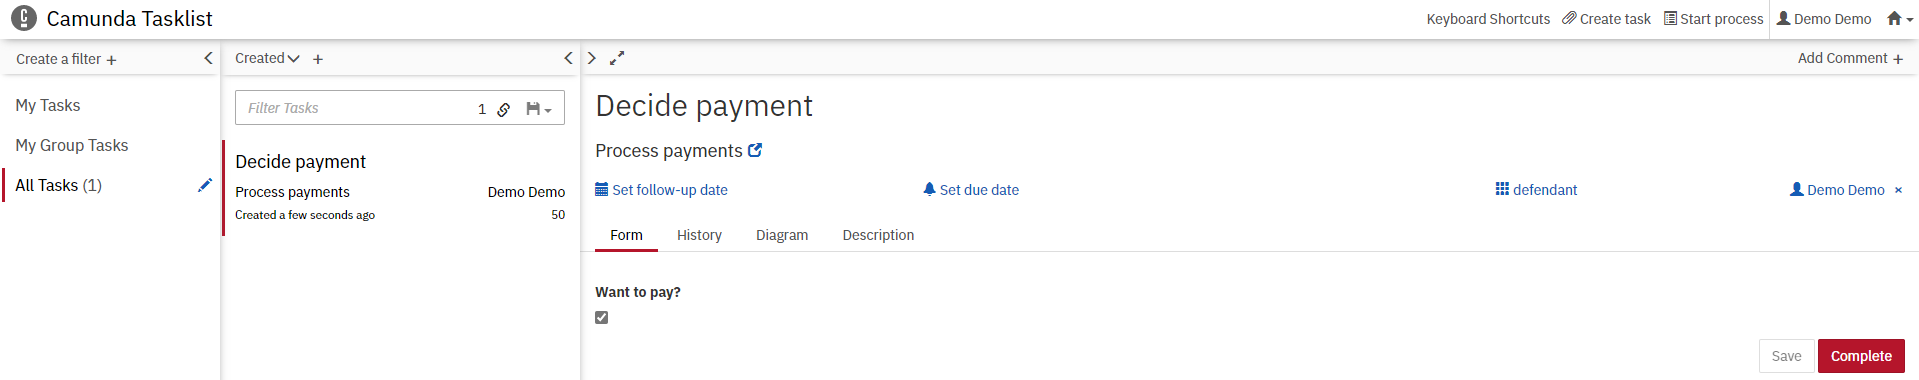
\includegraphics[width=22cm]{pic/camunda4}
            \caption{BPMN form: Decide to pay}
            \label{fig:camunda4}
        \end{figure}
    
    \end{landscape}

\section{Results Presentation}\label{sec:presentation}

An url to our presentation video: \url{https://www.youtube.com/watch?v=qfprck_Djro}


%------------------------------------------------------------------------------------------
% Use bibtex to produce bibliography used in the project
%------------------------------------------------------------------------------------------
\bibliographystyle{plain}

\bibliography{main}

\end{document}
